\subsection{Check communication between master GBTx and MiniDAQ}
After programming the master GBTx board and verifying the return value, we can check
the communication between the GBTx and the MiniDAQ with \textbf{GBT Client}.

\begin{figure}[ht]
    \centering
    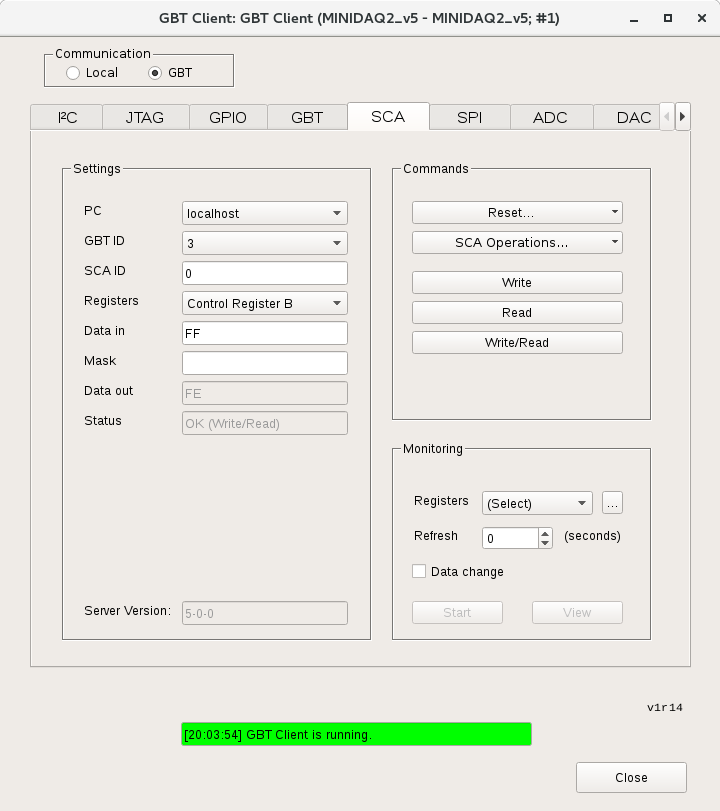
\includegraphics[width=0.9\textwidth]{res/gbt_client_master_gbt_sca_test.png}
    \caption{A typical UI for GBT Client, SCA tab.}
    \label{fig:sca-ui}
\end{figure}

Here we need to use the Linux server on the rack.
To launch that program, locate the \textbf{gedi} panel. Under
\textbf{LHCB framework},
click the \textbf{GBT Client}.
Choose \textbf{GBT} option under the \textbf{Communication} tab.
Navigate to \textbf{SCA} tab.

To check whether the link between GBTx and MiniDAQ is successfully established,
configure the parameters as shown in \autoref{fig:sca-ui},
changing \textbf{GBT ID} according to one's setup.

Now click \textbf{Write/Read}.
The \textbf{Data out} field should have a value of ``\texttt{FE}'', and the
\textbf{Status} should be ``OK (Write/Read)''.

\begin{leftbar}
    \textbf{GBT ID} corresponds to the physical optical link that is connected
    to the master GBTx board.
    Recall that in our setup, the master is connected to optical fiber 8, which
    is mapped to GBT channel 3.
\end{leftbar}

\begin{leftbar}
    There are only 4 \textbf{Registers}.
    All 4 registers work, the ``Control Register B'' is chosen for no apparent
    reason.
    What matters is the return value should be consistent with our expectation.
\end{leftbar}
